% Restored from Encyclopedia Section 5.4; normalization and boundary proof
% independently derived. Supplies an exact family at every weight.
\subsection{Unequal-ratio triangles and sharpness at every weight}
\label{sec:restored-OO-triangles}

The preceding common quarter-turn family has equal contraction
ratios. Opposite similarities also give an exact boundary family
covering every weight $0<w<1$.

\begin{theorem}[An exact triangle on every weighted inner bound]
\label{thm:restored-OO-triangles}
Let $0<\theta<\pi/2$, put $c=\cos\theta\,e^{i\theta}$, and define
\[
 g_0(z)=c\overline z,\qquad
 g_1(z)=c+(1-c)\overline z.
\]
Their attractor is the right triangle
$T_\theta=\operatorname{conv}\{0,1,c\}$. The two pieces have disjoint
interiors and meet precisely in the altitude
$[c,\cos^2\theta]$.

The normalized opposite--opposite coefficients are
\begin{equation}\label{eq:restored-triangle-coefficients}
 a=-\cos\theta\,e^{-3i\theta},\qquad
 b=i\sin\theta\,e^{-3i\theta}.
\end{equation}
One atlas representative is
\begin{equation}\label{eq:restored-triangle-atlas}
 \alpha=\frac\pi4,\qquad
 \gamma=3\theta-\frac{3\pi}4,\qquad
 w=\frac{\cos\theta}{\cos\theta+\sin\theta},\qquad
 \rho=\frac2{\cos\theta+\sin\theta}.
\end{equation}
Every parameter in this family belongs to the boundary of the
full opposite--opposite connectedness locus and to the boundary
relative to its fixed-weight parameter space.

As $\theta$ ranges over $(0,\pi/2)$, the weight ranges over $(0,1)$,
and the boundary radius is exactly
\[
 \rho=2\sqrt{w^2+(1-w)^2}.
\]
Thus the universal connected-core bound is sharp, uniformly over
the phases, at every fixed weight in the opposite--opposite class.
\end{theorem}

\begin{proof}
Write $c=x+iy$. Then $x=\cos^2\theta$, $y=\cos\theta\sin\theta>0$,
and $x^2+y^2=x$. Direct substitution gives
\[
 g_0(0,1,c)=(0,c,x),\qquad
 g_1(0,1,c)=(c,1,x).
\]
The identity $\operatorname{Re}(c\overline{(c-1)})=0$ says that
$T_\theta$ has its right angle at $c$. The two image triangles
partition it along the altitude from $c$ to $x$. Uniqueness of
the compact invariant set gives the asserted attractor and contact.

For clarity, compute the normalization explicitly. The average map
is $G(z)=c/2+\overline z/2$, whose fixed point is
$m=x+iy/3$. With $d=g_1(m)-m$ one obtains
\[
 d=\frac y3\bigl(2y+i(1-2x)\bigr)
   =-\frac{iy}{3}e^{2i\theta},\qquad
 \frac{\overline d}{d}=-e^{-4i\theta}.
\]
Under $H(z)=(z-m)/d$, the conjugated maps have constant terms $-1$ and $1$.
An opposite multiplier $u$ becomes $u\overline d/d$; applying this
to $c$ and $1-c=-i\sin\theta\,e^{i\theta}$ proves
\eqref{eq:restored-triangle-coefficients}. The moduli and arguments
give \eqref{eq:restored-triangle-atlas}, with the usual phase-lattice
identifications.

To prove boundary membership, consider, for $0<t\le1$,
\[
 g_{0,t}(z)=tc\overline z,\qquad
 g_{1,t}(z)=c+t(1-c)\overline z.
\]
Their images of $T_\theta$ remain in $T_\theta$: they shrink the
two subtriangles toward $0$ and $c$, respectively. For $t<1$,
the first lies in $\{\operatorname{Re}z\le tx\}$ and the second
in $\{\operatorname{Re}z\ge x\}$. Since $x>0$, the two pieces
are separated. Their attractor, which lies in $T_\theta$, is
therefore disconnected.

The normalized coefficient pairs depend continuously on $t$.
Indeed, the mean-map fixed point depends continuously on $t$,
and its normalizing difference is nonzero because $g_{0,t}$ fixes
$0$ while $g_{1,t}(0)=c\ne0$. Their contraction ratios are
$t\cos\theta$ and $t\sin\theta$, so their weight is independent
of $t$, while their radius is
$2/[t(\cos\theta+\sin\theta)]$.
The disconnected normalized parameters converge to the connected
triangle as $t\uparrow1$, proving both boundary assertions.

Finally, $w=(1+\tan\theta)^{-1}$ ranges bijectively over $(0,1)$,
and
$w^2+(1-w)^2=(\cos\theta+\sin\theta)^{-2}$.
The disconnected sequence at the same weight has radii decreasing
to this inner bound. Hence no larger radius can provide a
connectedness guarantee uniformly over the phases at that weight.
\end{proof}

At $\theta=\pi/4$, the normalized coefficients are
$a=(1+i)/2$, $b=(1-i)/2$, and the normalized triangle and contact are
\[
 K=\operatorname{conv}\{-3-i,\,3-i,\,2i\},\qquad Q=[-i,2i].
\]
This supplies an exact opposite--opposite landmark at
$(\alpha,\gamma,w,\rho)=(\pi/4,0,1/2,\sqrt2)$.

\begin{figure}[tbp]
\centering
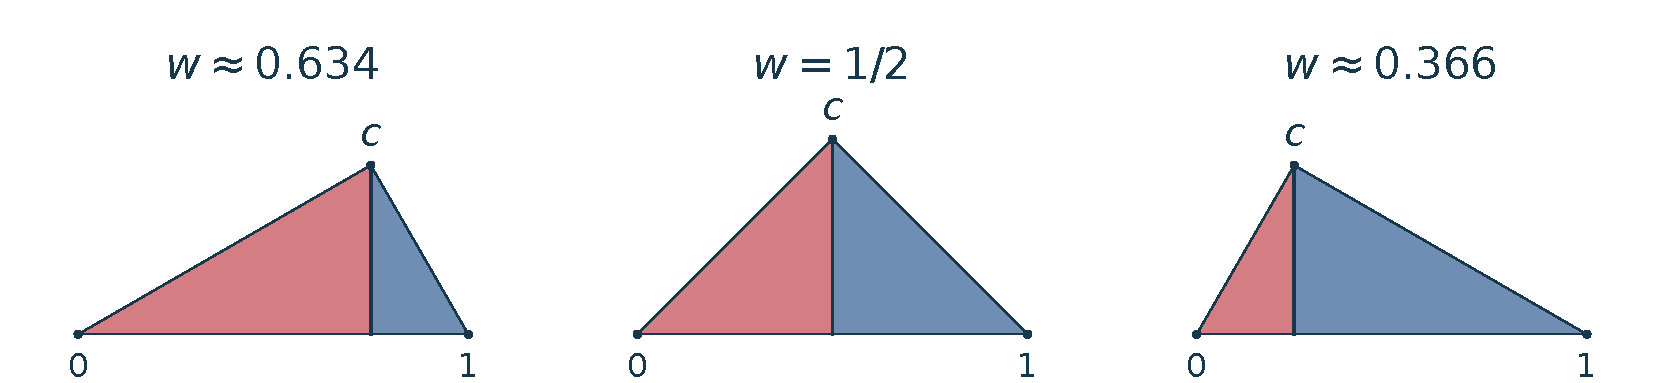
\includegraphics[width=\linewidth]{figures/triangle_contact_family.pdf}
\caption{The unequal-ratio opposite triangle family in endpoint coordinates,
with $\theta=\pi/6,\pi/4,\pi/3$. The two pieces meet along the altitude.
After canonical normalization, every triangle lies at
$\rho=2\sqrt{w^2+(1-w)^2}$; Theorem~\ref{thm:restored-OO-triangles}
proves boundary membership and sharpness for every $0<w<1$.}
\label{fig:triangles}
\end{figure}
